\documentclass{article}

\def\ParSkip{} 
% Packages
\usepackage{amssymb,amsmath,amsthm,bbm}
\usepackage{verbatim,float,url,dsfont}
\usepackage{graphicx,subfigure,psfrag}
\usepackage{algorithm,algorithmic}
\usepackage{mathtools,enumitem}
\usepackage{multirow}
\usepackage{ragged2e}
\usepackage{xr-hyper}
\usepackage{array}

\usepackage[colorlinks=true,citecolor=blue,urlcolor=blue,linkcolor=blue]{hyperref}
\usepackage[margin=1in]{geometry}
\usepackage[round]{natbib}

\usepackage[utf8]{inputenc} % allow utf-8 input
\usepackage[T1]{fontenc}    % use 8-bit T1 fonts
\usepackage{booktabs}       % professional-quality tables
\usepackage{nicefrac}         % compact symbols for 1/2, etc.
\usepackage{microtype}      % microtypography

\ifdefined\TimesFont 
\usepackage{times} % use times font
\fi

\ifdefined\ParSkip 
\usepackage{parskip} % use par skip
\fi

% Theorems and such
\newtheorem{theorem}{Theorem}
\newtheorem{lemma}{Lemma}
\newtheorem{corollary}{Corollary}
\newtheorem{proposition}{Proposition}
\theoremstyle{definition}
\newtheorem{remark}{Remark}
\newtheorem{definition}{Definition}

% Assumption
\newtheorem*{assumption*}{\assumptionnumber}
\providecommand{\assumptionnumber}{}
\makeatletter
\newenvironment{assumption}[2]{
  \renewcommand{\assumptionnumber}{Assumption #1#2}
  \begin{assumption*}
  \protected@edef\@currentlabel{#1#2}}
{\end{assumption*}}
\makeatother

% Widebar
\makeatletter
\newcommand*\rel@kern[1]{\kern#1\dimexpr\macc@kerna}
\newcommand*\widebar[1]{%
  \begingroup
  \def\mathaccent##1##2{%
    \rel@kern{0.8}%
    \overline{\rel@kern{-0.8}\macc@nucleus\rel@kern{0.2}}%
    \rel@kern{-0.2}%
  }%
  \macc@depth\@ne
  \let\math@bgroup\@empty \let\math@egroup\macc@set@skewchar
  \mathsurround\z@ \frozen@everymath{\mathgroup\macc@group\relax}%
  \macc@set@skewchar\relax
  \let\mathaccentV\macc@nested@a
  \macc@nested@a\relax111{#1}%
  \endgroup
}
\makeatother

% Min and max 
\DeclareMathOperator*{\argmin}{argmin}
\DeclareMathOperator*{\argmax}{argmax}
\DeclareMathOperator*{\minimize}{minimize}
\DeclareMathOperator*{\maximize}{maximize}
\DeclareMathOperator*{\find}{find}
\DeclareMathOperator{\st}{subject\,\,to}

% Other operators
\DeclareMathOperator{\Cov}{Cov}
\DeclareMathOperator{\Var}{Var}
\DeclareMathOperator{\dm}{dim}
\DeclareMathOperator{\col}{col}
\DeclareMathOperator{\row}{row}
\DeclareMathOperator{\nul}{null}
\DeclareMathOperator{\rank}{rank}
\DeclareMathOperator{\nuli}{nullity}
\DeclareMathOperator{\spa}{span}
\DeclareMathOperator{\sign}{sign}
\DeclareMathOperator{\supp}{supp}
\DeclareMathOperator{\diag}{diag}
\DeclareMathOperator{\aff}{aff}
\DeclareMathOperator{\conv}{conv}
\DeclareMathOperator{\dom}{dom}
\DeclareMathOperator{\tr}{tr}
\DeclareMathOperator{\df}{df}

% Other shortcuts 
\def\R{\mathbb{R}}
\def\C{\mathbb{C}}
\def\E{\mathbb{E}}
\def\P{\mathbb{P}}
\def\T{\mathsf{T}}
\def\half{\frac{1}{2}}
\def\df{\mathrm{df}}
\def\hy{\hat{y}}
\def\hf{\hat{f}}
\def\hmu{\hat{\mu}}
\def\halpha{\hat{\alpha}}
\def\hbeta{\hat{\beta}}
\def\htheta{\hat{\theta}}
\def\indep{\perp\!\!\!\perp}
\def\th{^{\textnormal{th}}}

\def\cA{\mathcal{A}}
\def\cB{\mathcal{B}}
\def\cD{\mathcal{D}}
\def\cE{\mathcal{E}}
\def\cF{\mathcal{F}}
\def\cG{\mathcal{G}}
\def\cK{\mathcal{K}}
\def\cH{\mathcal{H}}
\def\cI{\mathcal{I}}
\def\cL{\mathcal{L}}
\def\cM{\mathcal{M}}
\def\cN{\mathcal{N}}
\def\cP{\mathcal{P}}
\def\cS{\mathcal{S}}
\def\cT{\mathcal{T}}
\def\cW{\mathcal{W}}
\def\cX{\mathcal{X}}
\def\cY{\mathcal{Y}}
\def\cZ{\mathcal{Z}}

\usepackage[normalem]{ulem}
\usepackage{centernot}

\title{Lecture 3: Regularization and Smoothing \\ \smallskip  
\large Introduction to Time Series, Fall 2023 \\ \smallskip
Ryan Tibshirani}
\date{}

\begin{document}
\maketitle
\RaggedRight
\vspace{-50pt}

\section{Trouble in high dimensions?} 

\def\new{\text{new}}

\begin{itemize}
\item As in the regression lecture, let's suppose that we seek $\beta \in \R^p$  
  such that for given samples $x_i \in \R^p$ and $y_i \in \R$ (predictor and
  response pairs), $i = 1,\dots,n$,    
  \[
  y_i \approx x_i^\T \beta, \quad  i = 1,\dots,n 
  \]
  (As explained in that lecture, our notation omits the intercept from the
  model, but that is done without a loss of generality, since it can always be
  obtained by appending a coordinate value of 1 to the start of each $x_i$) 

\item Equivalently, we can write $y \in \R^n$ for the response vector (with
  $i\th$ component $y_i$) and $X \in \R^{n \times p}$ for the feature matrix
  (with $i\th$ row $x_i)$, and say that we are seeking $\beta$ such that $y
  \approx X \beta$ 

\item Recall, the least squares estimates of the coefficients are given by
  solving  
  \begin{equation}
  \label{eq:ls}
  \min_{\beta \in \R^p} \, \sum_{i=1}^n (y_i - x_i^\T \beta)^2 \iff
  \min_{\beta \in \R^p} \, \|y - X \beta\|_2^2
  \end{equation}
  where we use $\|\cdot\|_2$ for the Euclidean or $\ell_2$ norm of a vector,
  defined for $a \in \R^d$ as \smash{$\|a\|_2^2 = \sum_{i=1}^d a_i^2$}

\item If $p \leq n$ and $\rank(X) = p$ (here $\rank(X)$ denotes the rank of the 
  matrix $X$), then this produces the unique solution    
  \begin{equation}
  \label{eq:coef}
  \hbeta = (X^\T X)^{-1} X^\T y  
  \end{equation}

\item But if $p > n$, which means we have more features than samples, which we 
  often call the ``high dimensional'' (or ``overparametrized'') setting, then we 
  are in trouble ... the matrix $X^\T X$ cannot be invertible, so the expression
  in \eqref{eq:coef} isn't even well-defined   

\item Moreover, the least squares optimization problem \eqref{eq:ls} does not
  have a unique solution in this case. Indeed, are you'll show on the homework,
  it \smash{$\tilde\beta$} is one solution, then any other vector of the form    
  \begin{equation}
  \label{eq:coef_eta}
  \hbeta = \tilde\beta + \eta, \quad \text{where $\eta \in \nul(X)$}
  \end{equation}
  also solves \eqref{eq:ls}, where $\nul(X)$ is the null space of the matrix
  $X$:
  \[
  \nul(X) = \{ \eta \in \R^p : X \eta = 0 \} 
  \]

\item When $\rank(X) < p$, the null space $\nul(X)$ is nonempty, and since it 
  is a linear space: $\eta \in \nul(X) \implies c \eta \in \nul(X)$ for any $c
  \in \R$, we see that from one least squares solution \smash{$\tilde\beta$}, we
  can generate \emph{infinitely many others} in \eqref{eq:coef_eta} 
  
\item Furthermore, we can always take the ``one least squares solution'' to be:  
  \begin{equation}
  \label{eq:coef_mn}
  \tilde\beta = (X^\T X)^+ X^\T y
  \end{equation}

  \item Here $A^+$ denotes the \emph{generalized inverse} (also called the 
  \emph{Moore-Penrose pseudoinverse}) of a matrix $A$. If you don't know what
  that is, then it doesn't really matter for this lecture, but you can think of
  it precisely as follows: among all solutions in \eqref{eq:ls}, the solution in
  \eqref{eq:coef_mn} is the unique one having the smallest $\ell_2$ norm 
  \smash{$\|\tilde\beta\|_2$} 

\item So, now we come to the discussion of specific \emph{troubles}. There are
  actually two distinct troubles. The first trouble involves the interpretation
  of the coefficients themselves. If we are interested in such interpretations,
  then the $p = n$ barrier is the end of the road for least squares. Why? Once
  $p > n$, and we find any least squares solution \smash{$\tilde\beta$} with
  \smash{$\tilde\beta_j > 0$} for some $j$, then we can always
  find\footnote{Technically, this is only true if $\nul(X) \not \perp e_j$,
    where $e_j$ is the $j\th$ standard basis vector.}  
  another solution \smash{$\hbeta$} of the form \eqref{eq:coef_eta} with
  \smash{$\hbeta_j < 0$}. You will prove this on the homework. Thus we cannot
  even consistently interpret the sign of any of any estimated coefficient (let
  alone its magnitude) 

\item The second trouble involves prediction. The $p = n$ barrier is generally
  disastrous for least squares prediction. If $p < n$ and \smash{$\hat{y}_{\new}
    = x_{\new}^\T \hbeta$} is the least squares prediction at a new predictor
  value \smash{$x_{\new}$} (for \smash{$\hbeta$} the usual least squares
  coefficients in \eqref{eq:coef}), whose associated response is
  \smash{$y_{\new}$}, then under fairly standard conditions for regression
  theory,
% \footnote{This assumes that the true model is linear and the errors are
%   independent of the features (as well as assuming that the data are all
%   i.i.d., and some other mild-ish conditions on the distributions of the
%   errors and features that are not worth mentioning). In other words, it is a
%   fairly idealized model. So the fact that least squares performs poorly here
%   as $p$ approaches $n$, in this model, is especially notable.} 
  the prediction MSE behaves as: 
  \[
  \E \big[ (y_{\new} - \hat{y}_{\new})^2 \big] \approx \sigma^2
  \frac{p}{n-p} 
  \]
  for large $n$ and $p$, where $\sigma^2$ is the error variance. What do we
  notice? This explodes as $p$ approaches $n$. Big problem!

\item (Aside: what happens with the prediction MSE when $p > n$? The answer may
  surprise you. The MSE associated with the particular solution in
  \eqref{eq:coef_mn} is actually quite interesting and in some ways exotic when 
  $p > n$. Typically we need $p$ to be \emph{much larger} than $n$ (away from
  the $p = n$ barrier) in order for it to be well-behaved. This has been the
  topic of a recent flurry of research in statistics in machine learning ...  we
  won't focus on it in this lecture and will instead talk about explicit
  regularization. But feel free to ask about it in office hours)    
\end{itemize}


\section{Regularization}

\begin{itemize}
\item \emph{Regularization} to the rescue! This will finesse both of the
  problems described above: it gives us a way to produce nontrivial coefficient 
  estimates, and it often gives us more accurate predictions 

\item In the regression setting, a general approach for regularization moves us 
  from \eqref{eq:ls} to solving:
  \begin{equation}
  \label{eq:ls_pen}
  \min_\beta \; \|y - X\beta\|_2^2 + h(\beta)
  \end{equation}

\item Here $h : \R^p \to \R_+$ is some (typically convex) penalty
  function. Arguably the three canonical choices for penalties are based on the
  $\ell_0$, $\ell_1$, and $\ell_2$ norms:  
  \begin{align*}
  h(\beta) &= \|\beta\|_0 = \sum_{j=1}^p 1\{\beta_j \not= 0\}, \\
  h(\beta) &= \|\beta\|_1 = \sum_{j=1}^p |\beta_j|, \\
  h(\beta) &= \|\beta\|_2^2 = \sum_{j=1}^p \beta_j^2.
  \end{align*}
  This gives rise to what we call \emph{best subset selection}, the
  \emph{lasso}, and \emph{ridge regression}, respectively

\item (Aside: calling $\|\cdot\|_0$ the ``$\ell_0$ norm'' is a misnomer, as it
  is not actually a norm: it does not satisfy positive homogeneity, i.e.,
  $\|a\beta\|_0 = a\|\beta\|_0$ for all $a>0$. It would be more accurate to
  call it the ``$\ell_0$ pseudonorm'', but nearly everybody just calls it the
  ``$\ell_0$ norm'')

\item Critically, $\|\cdot\|_0$ is \emph{not convex}, while $\|\cdot\|_1$ and 
  $\|\cdot\|_2$ are convex (note that any norm is a convex function). This makes
  best subset selection a nonconvex problem, and one that is generally very hard
  to solve in practice except for small $p$. We won't focus on best subset 
  selection further in this lecture. (Though it is itself the topic of a flurry 
  of work in the operations research literature a few years ago ... which you
  can ask about in office hours if you are curious) 
\end{itemize}

\subsection{Ridge}

\begin{itemize}
\item The \emph{ridge} estimates of regression coefficients are given by solving    
  \[
  \min_{\beta \in \R^p} \, \sum_{i=1}^n (y_i - x_i^\T \beta)^2 + \lambda
  \sum_{j=1}^p \beta_j^2
  \]
  or equivalently
  \begin{equation}
  \label{eq:ridge}
  \min_{\beta \in \R^p} \, \|y - X \beta\|_2^2 + \lambda \|\beta\|_2^2
  \end{equation}

\item Here $\lambda \geq 0$ is a tuning parameter (also called the
  regularization parameter) which trades off the importance of the squared
  loss---first term in \eqref{eq:ridge}, with the ridge penalty---second term in
  \eqref{eq:ridge}. In other words, the larger the value of $\lambda$, the more
  weight we put on the ridge penalty, which penalizes large coefficient
  magnitudes very heavily. This results in estimates that we call more
  ``regularized''  

\item The solution in \eqref{eq:ridge} has an explicit form (derived by
  differentiating the criterion and setting the result equal to zero), 
  \begin{equation}
  \label{eq:coef_ridge}
  \hbeta = (X^\T X + \lambda I)^{-1} X^\T y
  \end{equation}
  where $I$ is in the $p \times p$ identity matrix. This \emph{always exists}
  (the matrix $X^\T X + \lambda I$ is always invertible), regardless of the
  relative sizes of $n,p$
\end{itemize}

\subsection{Lasso}

\begin{itemize}
\item The \emph{lasso} estimates of regression coefficients are given by solving    
  \[
  \min_{\beta \in \R^p} \, \sum_{i=1}^n (y_i - x_i^\T \beta)^2 + \lambda
  \sum_{j=1}^p |\beta_j|
  \]
  or equivalently
  \begin{equation}
  \label{eq:lasso}
  \min_{\beta \in \R^p} \, \|y - X \beta\|_2^2 + \lambda \|\beta\|_1
  \end{equation}

\item Again, $\lambda \geq 0$ is a tuning parameter trading off the importance 
  of the squared loss and the $\ell_1$ penalty---first and second terms in
  \eqref{eq:lasso}. As before, larger $\lambda$ gives us more regularized
  estimates 

\item There are a number of key differences between the ridge \eqref{eq:ridge}
  and \eqref{eq:lasso} problems (and estimator). First, the lasso problem does
  not have a closed-form solution (it does not even necessarily always admit a
  unique solution; though it is essentially always unique if we have
  continuously distributed features)

\item A second key difference is that the lasso estimates of the regression
  coefficients are \emph{sparse}. In other words, solving the lasso problem
  results in a vector \smash{$\hbeta$} with many components exactly equal to
  zero, and a larger choice of $\lambda$ will result in more zeros. This doesn't
  happen with ridge regression, whose coefficient estimates are generically
  \emph{dense}. Figure \ref{fig:lasso_ridge} is the ``classic'' picture used to
  explain this, and we will talk through its interpretation in lecture

\begin{figure}[htb]
\centering
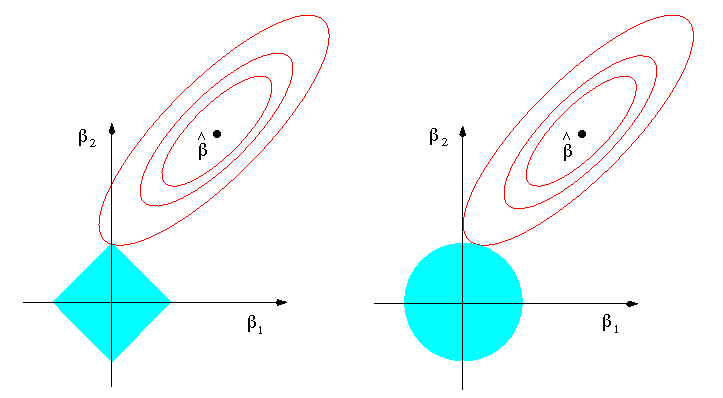
\includegraphics[width=0.95\textwidth]{lasso_ridge.pdf}
\caption{\it The ``classic'' illustration comparing lasso and ridge, each in
  constrained form (from ``Elements of Statistical Learning'' by Hastie,
  Tibshirani, and Friedman)}
\label{fig:lasso_ridge}
\end{figure}

\item Importantly, this allows the lasso to perform \emph{variable selection}
  in the working linear model. By zero-ing out some coefficients exactly, it
  discards some features from having any predictive influence in the fitted
  model. Which precise features it discards is chosen based on the data. Many
  people like sparsity because it leads to better interpretability    
\end{itemize}

\subsection{Discussion}

\begin{itemize}
\item We should be clear that the lasso is not ``better'' than ridge, in any
  general sense, and neither is ridge ``better'' than the lasso. They each can
  help tremendously with stabilizing coefficient estimates so as to lead to
  improved predictive accuracy. They each do so by regularizing in different
  ways 

\item The most basic question to ask: is a sparse linear model likely
  to be a good (or desirable) approximation to the true regression function? If
  so, then the lasso can outperform (or be preferable) to ridge. On the other 
  hand, in problems where there are many underlying features that are relevant
  for prediction, ridge can outperform the lasso 

\item (And often times people combine the two penalties which gives rise to the
  \emph{elastic net}) 

\item There is a lot more to say---in terms of connections to other ideas in
  statistics, extensions, and so on---but we won't be able to cover it in this
  class. We'll simply view ridge and lasso as tools that allow us to consider 
  many more features than we would otherwise feel comfortable including in
  traditional regression models, and then regularize in order to control
  variance (stabilize estimates)   

\item In time series regression, in the vein of examples we studied in the last 
  lecture, this would allow us to include \emph{many lags} of a feature of
  interest, or a few lags of \emph{many external covariates}, and so on, and
  then apply a ridge or lasso penalty. Then, you might wonder: how would we
  select $\lambda$? In fact, you already know the answer (for problems with a
  predictive focus): use time series cross-validation!

\item That is, define a grid of $\lambda$ values, fit ridge or lasso estimates
  for each $\lambda$, let each one make predictions, and select the value that 
  yields the best CV error. You will practice this on the homework, where you'll
  also use the \verb|glmnet| package to solve the ridge and lasso problems 
\end{itemize}

\section{Smoothing}

\subsection{Linear filters}

\subsection{Hodrick-Prescott filter}

\subsection{Trend filter}

% HP filter
% Trend filter

\end{document}
